PMTs were used in TRITIUM experiment for two main objectives. On the one hand, to know the amount of incident photons that reach the PMT photocathode, which is important to characterize fibers, and, on the other hand, to know the energy of events, which allows us to discriminate events according to their origin, obtaining an energy spectrum of triggered events. 

To know the amount of photons that reach the photocathode, the PMT should work without internal gain since it introduces a large uncertainty in the measurement. For that end, the electron multiplication stage (shown in section \ref{subsubsec:PMTs}) should not be employed. This was achieved with the help of a PCB, shown in Figure \ref{fig:ElectronicSchemeBasePMTNoGain}, designed, built and tested for this purpose.  

\begin{figure}[htbp]
\centering
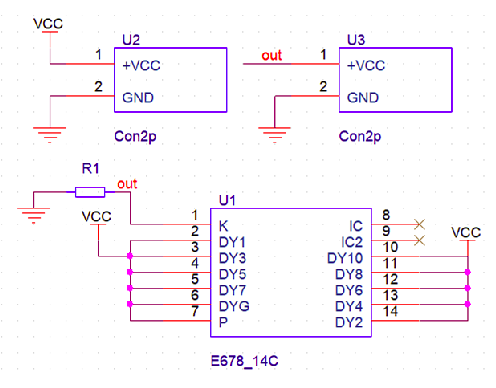
\includegraphics[scale=0.5]{3DesignPrinciples/32Tritium_detector/ElectronicSchemBasePMTNoGain.png}
\caption{Electronic scheme of the voltage divider circuit used for working with PMTs without internal gain).\label{fig:ElectronicSchemeBasePMTNoGain}}
\end{figure}

This PCB short-circuits the dynodes and reads the signal directly from the photocathode. This PCB was designed to be supplied with a positive voltage smaller than the usual running voltage because this voltage is only needed to create a voltage difference between the photocathode and the first dinode. As the electrons are not multiplied, the output pulse of the photosensor is very small (currents of the order of tens of nanoamperes) and a special readout system is needed. The chosen system is Keithley 6487 Picoammeter/Voltage Source \cite{DataSheetKeithley6487}, a commercial system from Keithley. This system has some useful options such as automatic baseline correction, the ability to read currents of the order of picoamperes and the possibility of carrying out mathematical operation on the signal, such as the average of N measurements with the associated statistical error, where N is programmable by the user ($N=100$ in all our studies). Finally, the number of photons reaching the photocathode is calculated from,
\begin{equation}
Nº\gamma/\sec = \frac{\left( I_{PMT} - I_{DC} \right)}{q_e \cdot{} QE \cdot{} CE}
\label{eq:NumPhotonsFromIntensityPMT}
\end{equation}
where $I_{PMT}$ is the output current of the PMT when it detects photons and $I_{DC}$ is the dark current. This equation takes into account the quantum efficiency of the PMT, which is close to $30\%$, and the capture efficiency in the dynodes, equal to 1 since the signal is read directly from the photocathode. In addition, it is assumed that each detected photon only generates one electron, the charge of which is $q_e$. To determine the energy of the events, the gain of the PMT has to be restored by removing the short-circuit of the electron multiplication stage. The number of PMTs used simultaneously was one, two or four, depending on the measurement. A simplified scheme of the electronic chain employed in each case is shown in Figures \ref{subfig:ElectronicConfiguraiton1PMT}, \ref{subfig:ElectronicConfiguraiton2PMT} and \ref{subfig:ElectronicConfiguraiton4PMT}, based on various NIM modules\footnote{The Nuclear Instrumentation Module (NIM) is a standard specification convention for electrical and mechanical parameters defined in electronic modules used in experimental nuclear and particle physics.}.

\begin{figure}
\centering
    \begin{subfigure}[b]{1.0\textwidth}
    \centering
    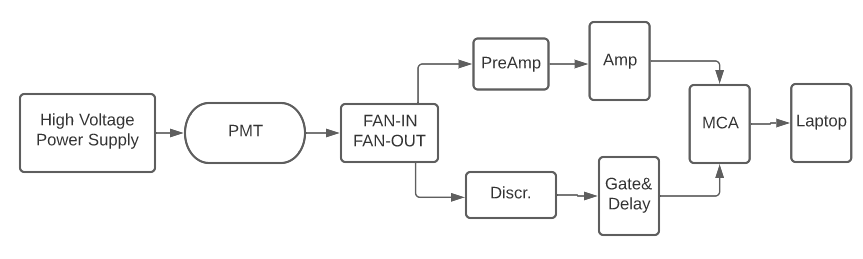
\includegraphics[width=\textwidth]{3DesignPrinciples/32Tritium_detector/Electronical_Scheme_1_PMT.png}  
    \caption{\label{subfig:ElectronicConfiguraiton1PMT}}
    \end{subfigure}
    \hfill
    \begin{subfigure}[b]{1.0\textwidth}
    \centering
    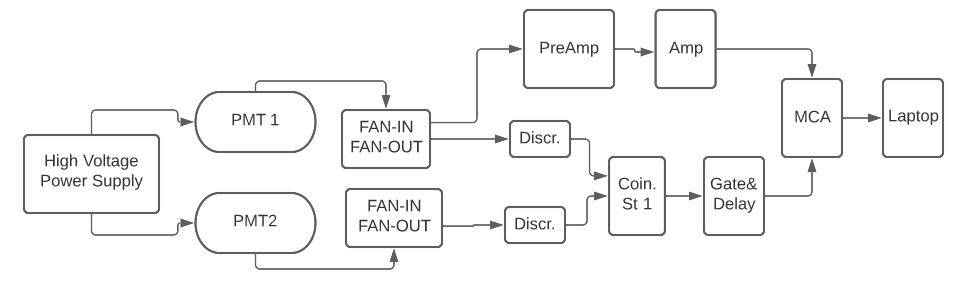
\includegraphics[width=\textwidth]{3DesignPrinciples/32Tritium_detector/Electronical_Scheme_2_PMTs.png}  
    \caption{\label{subfig:ElectronicConfiguraiton2PMT}}
    \end{subfigure}
    \hfill
    \begin{subfigure}[b]{1.0\textwidth}
    \centering
    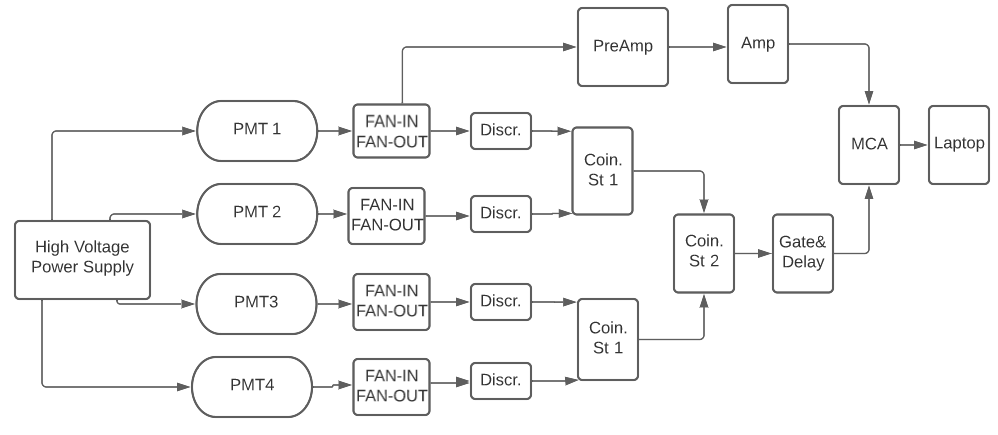
\includegraphics[width=\textwidth]{3DesignPrinciples/32Tritium_detector/Electronical_Scheme_4_PMTs.png}  
    \caption{\label{subfig:ElectronicConfiguraiton4PMT}}
    \end{subfigure}
 \caption{Schemes of the different electronic for measuring with PMTs. a) Employed when only one PMT is used. b) Employed when two PMTs are used in time coincidence. c) Employed when four PMTs are used in time coincidence.}
 \label{fig:ElectronicConfiguraitonsPMT}
\end{figure}

The PMTs were supplied in all the cases by TC 952 High Voltage Supply from Tennelec \cite{DataSheetHVSupplyTennelec}, which has four channels. If two or more configurations are needed, a second voltage supply HV Power Supply N 1130-4 from Wenzel Elektronik company \cite{DataSheetHVSupplyWenzel} with 4 additional channels, was employed. As it can be seen in the figures, there are two different lines followed by the PMT output signals, the amplification line, used to create an energy spectrum, and the time coincidence line, used to make time coincidences. Therefore, an analogic FAN IN-OUT module was used to duplicate the input signal. The module employed was the Quad linear FAN IN-OUT MODEL 740 from Philips Scintific \cite{DataSheetFANINOUT}, which has four channels. One output signal was used as the input for the amplification part and the second output was used as input for the time coincidence electronics.

\begin{enumerate}

\item{} The amplification line, which is the same for the three configurations, provides the energy information and is based on two steps;

%We have to take into accout that we have only used the signal from one PMT for the amplification part. We could have added a stage where we add the four PMT output signals and it would probably improve our results, but since our ultimate goal is to work with SiPM, we have not delved into that.

%The electronic path we have followed to achieve this amplification is:

\begin{enumerate}

\item{} The output signal is integrated by a preamplifier, which gives an output signal with a heigth proportional to the charge of the input pulse. This signal has a long tail\footnote{The length of the tail is, $\tau=RC$, where R is the input resistance and C is the capacitance used. It is the typical output signal in RC circuits.} produced by the preamplifier capacitance. The preamplifier used was "MODEL 9326 FAST PREAMP" from ORTEC \cite{DataSheetPreAmp}.

\item{} The output signal from the preamplifier is lead to the amplifier which gives a gaussian shaped output signal. The amplifier modules were 575A and 671 from ORTEC \cite{DataSheet575Amp, DataSheet671Amp}. An example of the output signal for 575A module is shown in Figure \ref{fig:InputSignalsMCA}, green color.

\end{enumerate}

\item{} The time coincidence line contains the time information and gives the gate that triggers coincident signals of both PMTs. This line consists of the following branches,

\begin{enumerate}

\item{} The output signal of the FAN IN-OUT module of each PMT is introduced into a discriminator module that gives a logic signal of $-1.2~\volt$ height and of $240~\nano\second$ width when a given threshold is exceeded. The discriminators employed are  Octuple Constant-Fraction Discriminator CF8000 module from ORTEC \cite{DataSheetDiscriminator} and 4 channels discriminator model 84 from CAEN \cite{DataSheetDiscriminatorCAEN}.

\item{} Time coincidences are required to ensure that detected events come from the scintillating fibers and to remove external light and dark current. The two logic signals given by the discriminator from the two PMTs that read a detector are introduced in a coincidence module which generates an output signal of $-1.4~\volt$ heigh and of $20~\ns$ width, when both imputs are in time coincidence. The modules used were Coincidence Unit Model 465 from LeCroy \cite{DataSheetCoincidenceLeCroy} and Coincidence Type N6234 from CERN-NP \cite{DataSheetCoincidenceCERN}.

\item{} Time coincidence of two different detectors (4 PMTs, configuration \ref{subfig:ElectronicConfiguraiton4PMT}) was also studied, which is useful to remove background due to hard cosmic radiation. To do so, a coincidence step similar to the previous one must be applied. The two single detector coincidence signal are checked for coincidence.

Some examples are shown in Figure \ref{fig:DifferentCoincidences} for time coincidences of two detectors (4 PMTs). There, four logical signals are shown, two of them (channel one and two, yellow and green respectively) come from two PMTs reading the first detector and the other two signals (channels three and four, color orange and violet respectively) come from PMTs reading the second detector.

\begin{enumerate}
\item{} In Figure \ref{subfig:signalInOnePMT} only one PMT (channel two) detected an event. It means that the event is likely not produecd in the scintillator. In this case, no output signal is generated.

\item{} In Figures \ref{subfig:signalInTwoPMTOneDetector} and \ref{subfig:signalInTwoPMTOtherDetector} two PMT signals of on of the detectors are generated but the other detector gives no signal. This event is discarded.

\item{} In Figure \ref{subfig:signalInAllPMTsBothDetector} the four signals are generated and, consequently, the output signal is generated and the event is recorded.

\begin{figure}
\centering
    \begin{subfigure}[b]{0.45\textwidth}
    \centering
    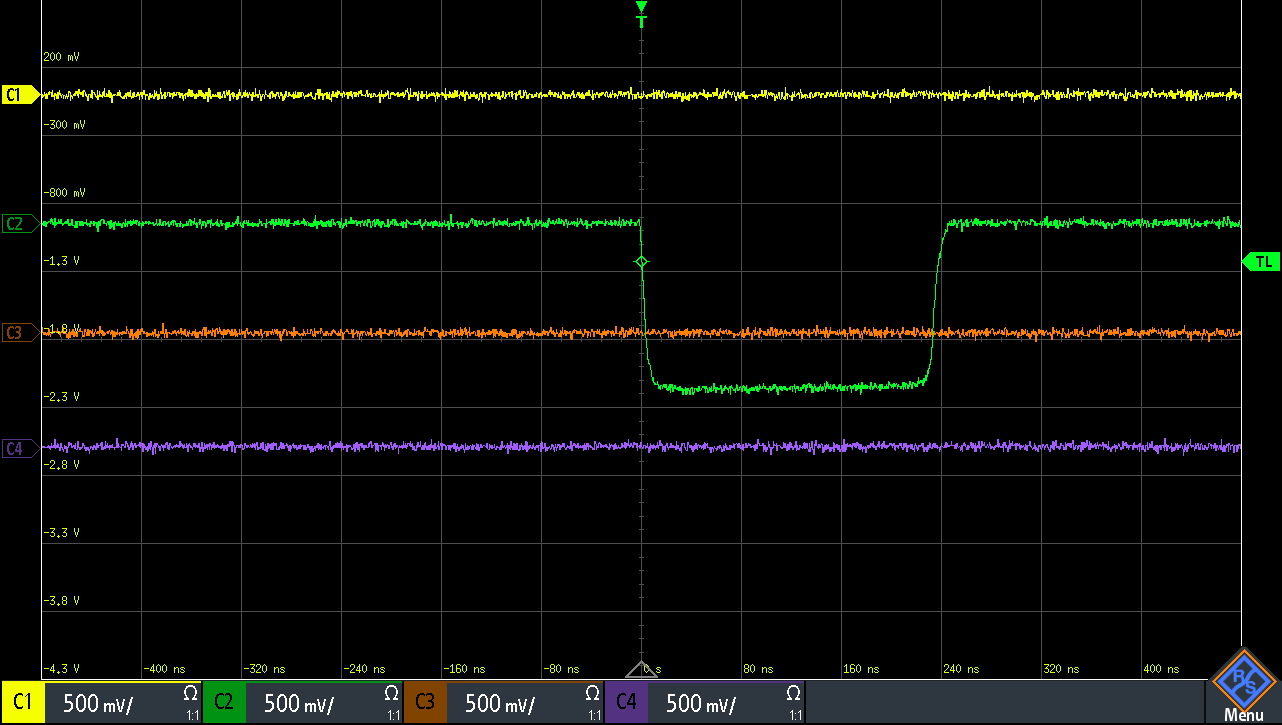
\includegraphics[width=\textwidth]{3DesignPrinciples/32Tritium_detector/1_coincidences.png}  
    \caption{\label{subfig:signalInOnePMT}}
    \end{subfigure}
    \hfill
    \begin{subfigure}[b]{0.45\textwidth}
    \centering
    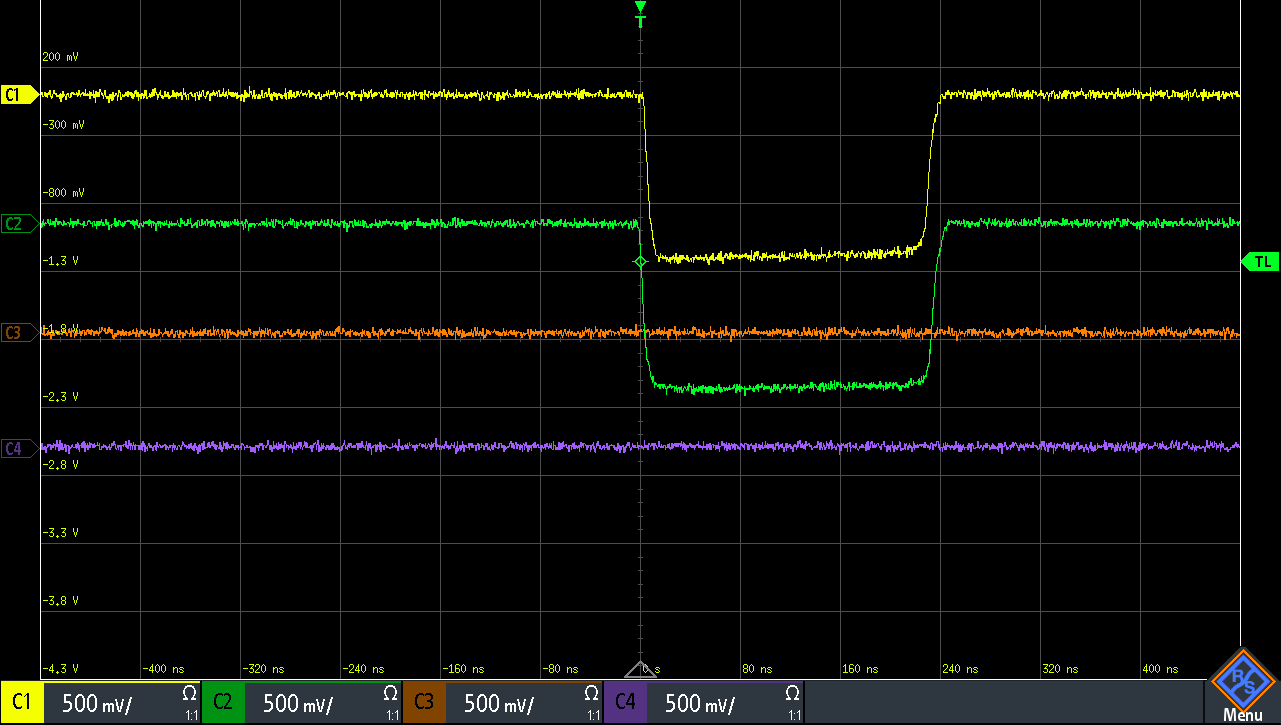
\includegraphics[width=\textwidth]{3DesignPrinciples/32Tritium_detector/2_coincidences_1.png}  
    \caption{\label{subfig:signalInTwoPMTOneDetector}}
    \end{subfigure}
    \hfill
    \begin{subfigure}[b]{0.45\textwidth}
    \centering
    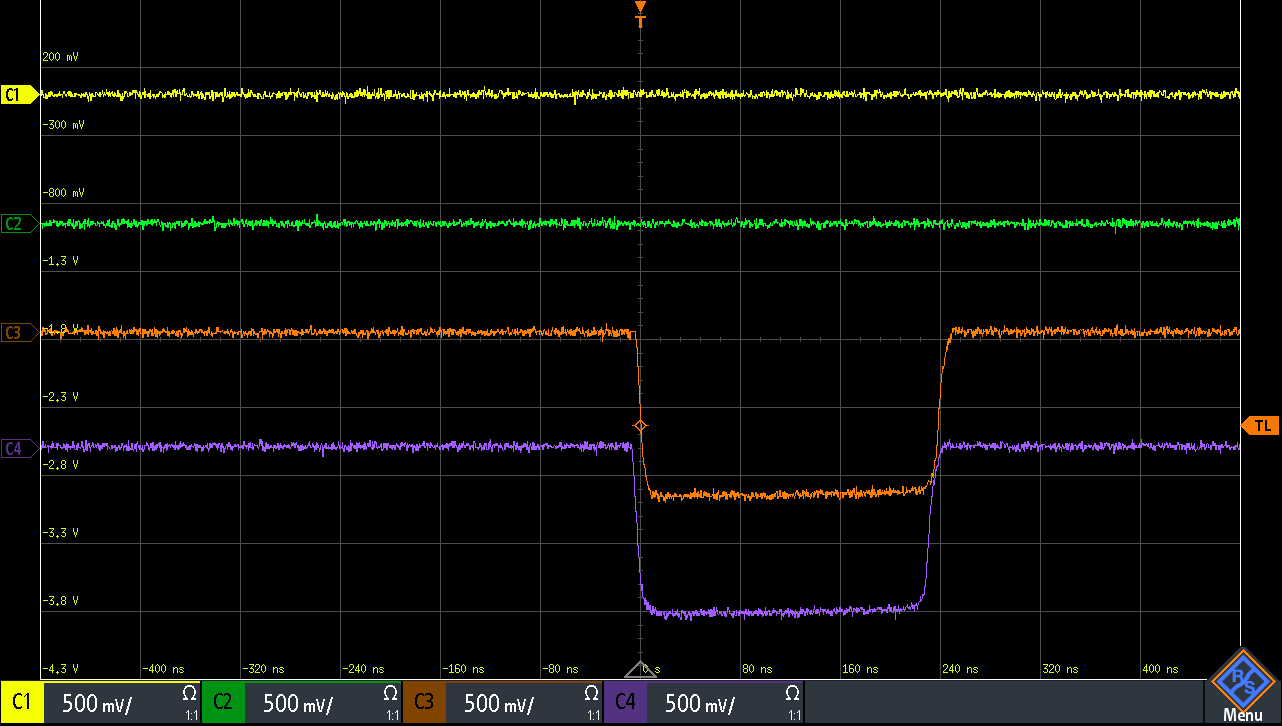
\includegraphics[width=\textwidth]{3DesignPrinciples/32Tritium_detector/2_coincidences_2.png}  
    \caption{\label{subfig:signalInTwoPMTOtherDetector}}
    \end{subfigure}
    \hfill
    \begin{subfigure}[b]{0.45\textwidth}
    \centering
    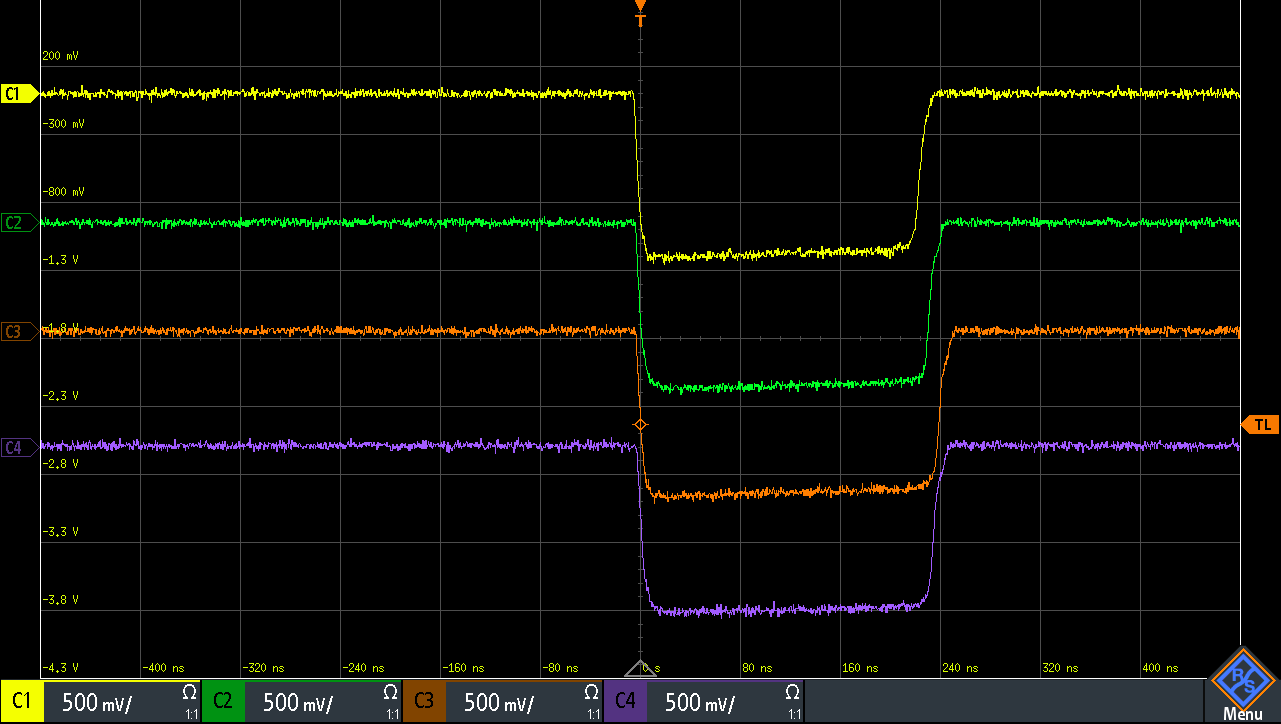
\includegraphics[width=\textwidth]{3DesignPrinciples/32Tritium_detector/4_coincidences.png}  
    \caption{\label{subfig:signalInAllPMTsBothDetector}}
    \end{subfigure}
 \caption{Different possibilities when time coincidences with PMTs are done. a) Event detected in only one PMT, one detector. b) Event detected in two PMTs, one detector. c) Event detected in two PMTs, other detector. d) Event detected in all PMTs, both detector.}
 \label{fig:DifferentCoincidences}
\end{figure}

\end{enumerate}

\item{} The logical output signal, is introduced in the Gate and Delay Generator, model 416A of the company ORTEC \cite{DataSheetGateAndDelay}, which gives a positive logical signal, called time windows, shown in Figure \ref{fig:InputSignalsMCA}, orange color, with a height of $8~\volt$ and width of $2~\mu\second$. This module is used to delay the time windows until it overlaps with the energy signal as it is shown in Figure \ref{fig:InputSignalsMCA}, orange signal.

\end{enumerate}

\end{enumerate}

As a final output of the electronics, a logical and analogical signals are obtained, shown in Figure \ref{fig:InputSignalsMCA}, which are recorded by the MCA 8000D, Pocket MCA from AMPTEK \cite{DataSheetMCA}. The analogical signal has information about the energy of the event and this is the signal which information is saved for later analysis. The logic signal (output from the Gate and Delay Generator module) indicates when the amplified signal must be saved.

\begin{figure}[htbp]
\centering
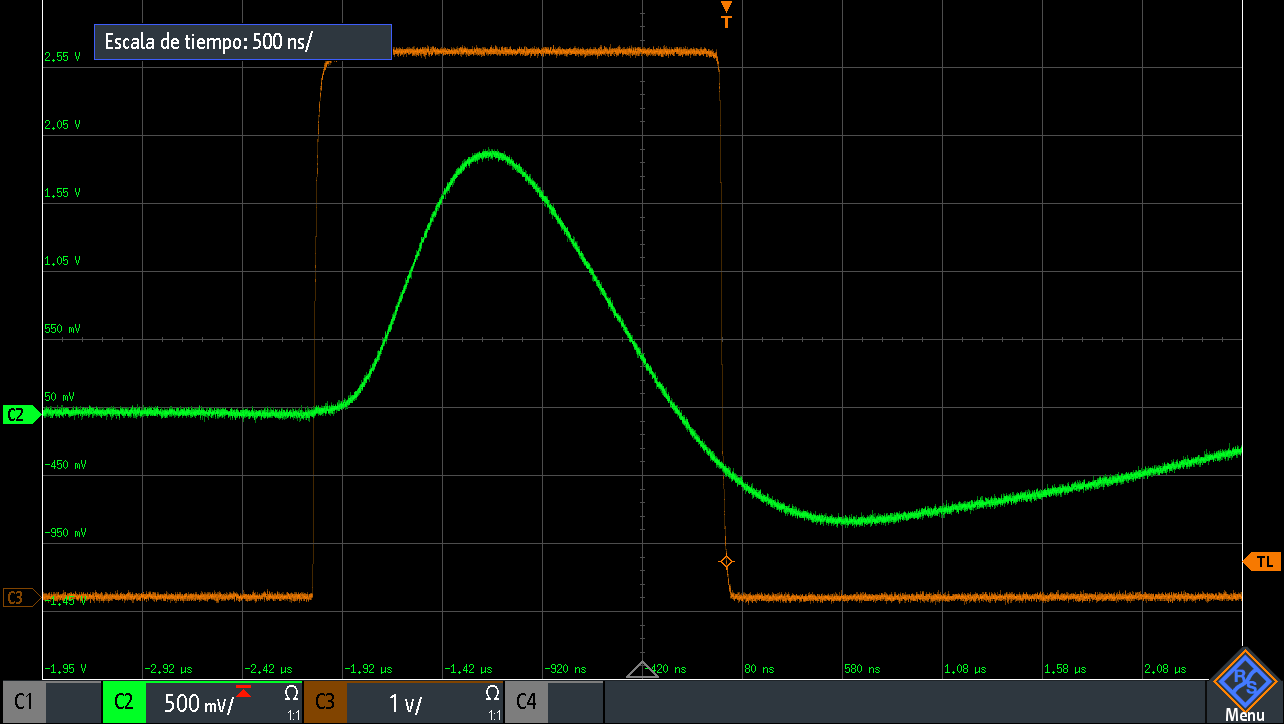
\includegraphics[scale=0.3]{3DesignPrinciples/32Tritium_detector/Input_MCA.png}
\caption{Signal amplified and logical gate (input signals of MCA).\label{fig:InputSignalsMCA}}
\end{figure}